Como primer paso, se conectó el cañon de electrones a la fuente de voltaje, para
así confirmar que esté funcionando correctamente, como se puede observar en la
\cref{fig:cañon-de-electrones}, a su vez, las bobinas de Helmholtz se
conectaron a la fuente de corriente.

\begin{figure}[htbp!]
  \centering
  \includegraphics[width=0.8\linewidth]{./images/Cañon.jpeg}
  \caption{Cañon de electrones en funcionamiento.}
  \label{fig:cañon-de-electrones}
\end{figure}

Una vez conectadas ambas fuentes se comenzó con la toma de datos, el voltaje
suministrado al cañon de electrones se varió entre 150 y \qty{350}{V},
mientras que la corriente en las bobinas se variaba entre 1 y \qty{3}{A}.
Para cada valor de voltaje, se hacian entre cuatro y cinco variaciones en la
corriente, para cada uno de estos se media un diámetro diferente que corresponde
a la circunferencia formada por el rayo de electrones debido a las bobinas,
esta circunferencia se puede observar en la \cref{fig:rayo-de-electrones}.
Para medir con mayor precisión estos valores, se conectó un voltímetro para el
cañon de electrones y un amperímetro para las bobinas de Helmholtz.

\begin{figure}[htbp!]
    \centering
    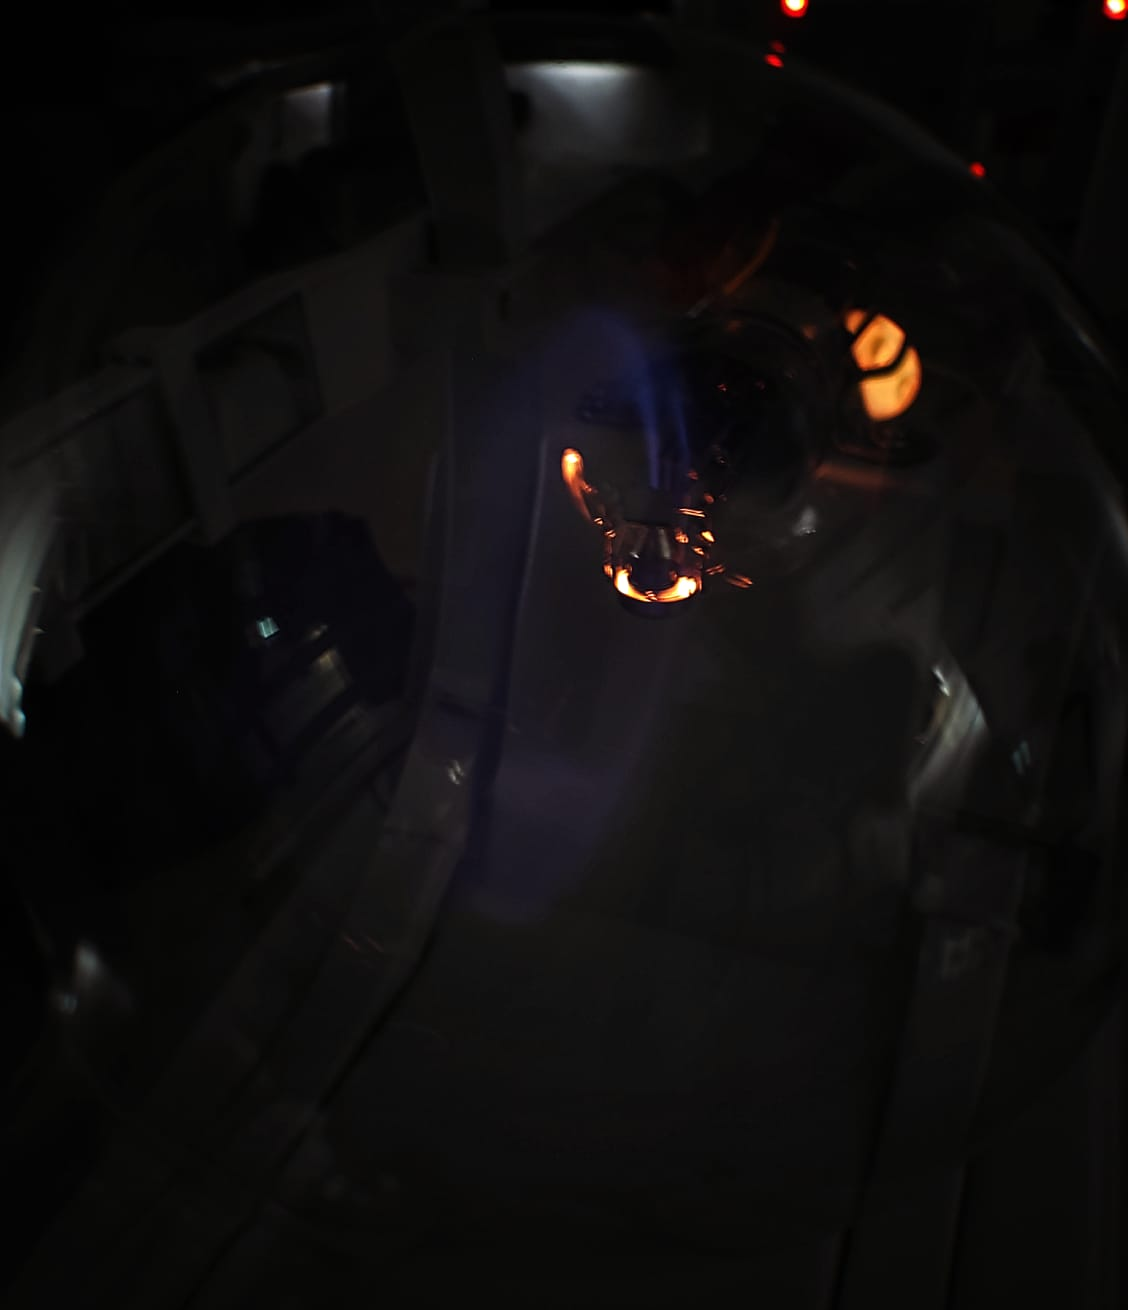
\includegraphics[width=0.8\linewidth]{./images/rayo-de-electrones.jpeg}
    \caption{Trayectoria del rayo de electrones.}
  \label{fig:rayo-de-electrones}
\end{figure}

Para medir estos radios, se usaron las dos regletas de plástico y cada una
tiene dos piezas de plástico movibles, ambas regletas ubicadas de forma paralela
la una con la otra y a su vez, deben estar ubicadas en el centro de las bobinas,
como se puede observar en la \cref{fig:reglas}.
Una de las piezas de plástico se colocan en un extremo de la circunferencia,
mientras que la otra se coloca en el extremo opuesto, y con ayuda de una regla
se mide la distancia entre ambas, la cual corresponde al diámetro de la
trayectoria con forma de circunferencia.

\begin{figure}[htbp!]
  \centering
  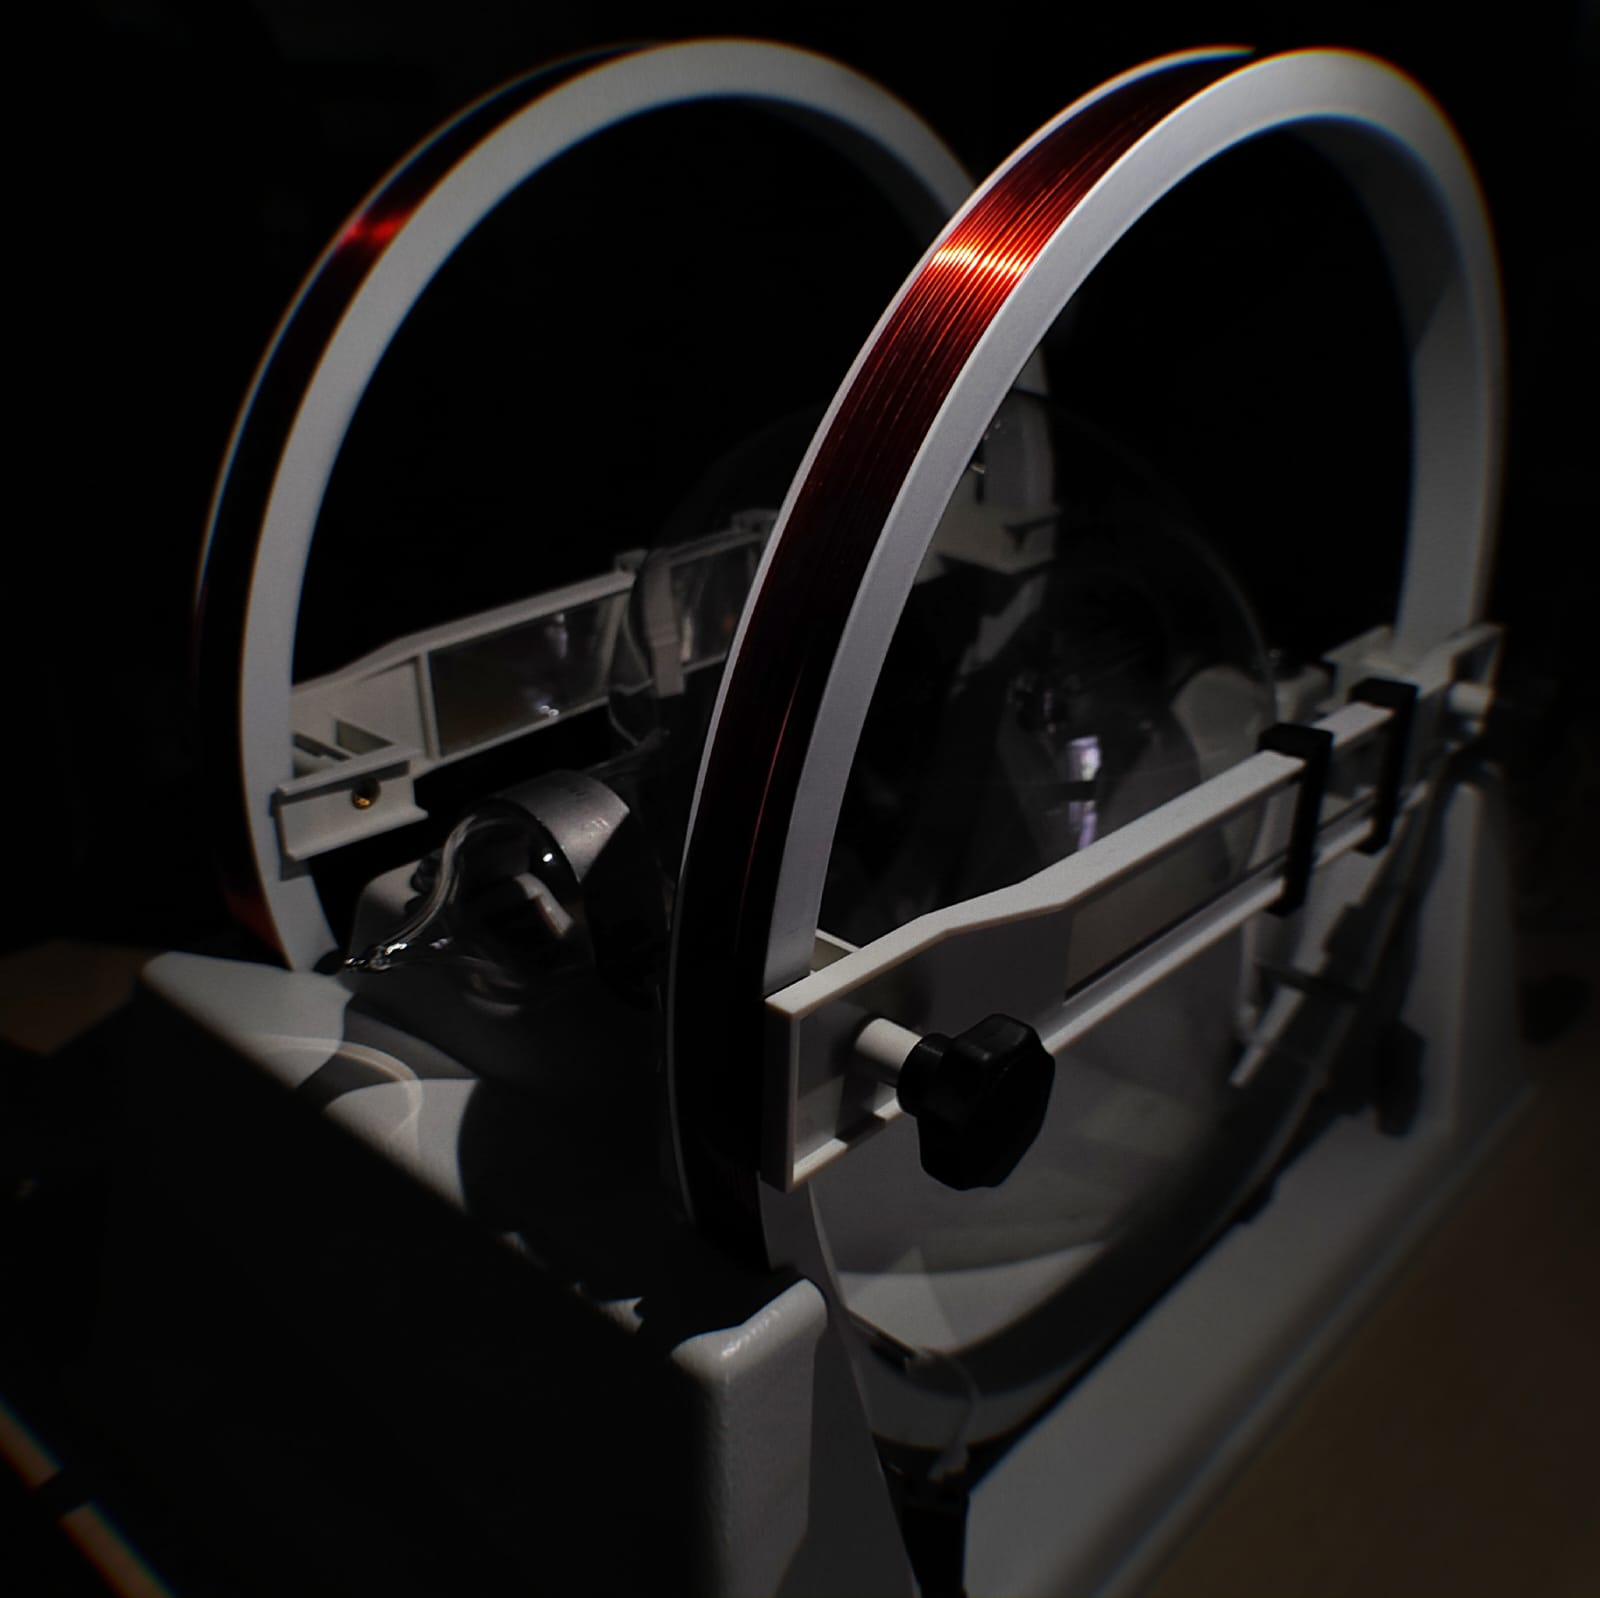
\includegraphics[width=0.8\linewidth]{./images/reglas.jpeg}
  \caption{Regletas de plástico.}
  \label{fig:reglas}
\end{figure}

Cada dato se guardó en una tabla para posteriormente hacer el calculo del valor
de la relación carga-masa.
